\subsection{\textit{Large-Scale Provisioning of
    Resource Constrained
    IoT Deployments, LEONORE}}
\label{subsec:leonore}

Riset ini menjelaskan mengenai cara pembuatan sebuah infrastruktur untuk melakukan \textit{provisioning} perangkat IoT dalam skala besar. Penelitian ini berfokus untuk membuat sebuah pendekatan terstruktur dalam menyediakan layanan \textit{deployment} lingkungan IoT dengan dua metode, yaitu \textit{Push} dan \textit{Pull}.

LEONORE dibuat untuk menyelesaikan tantangan, yaitu mengelola jutaan perangkat IoT yang heterogen pada sistem skala besar yang memiliki domain \textit{smart city}. Solusi yang sudah ada sering kali bersifat \textit{partial} ataupun manual dalam menangani sebagian infrastruktur. Tentunya, Hal ini tidak efisien dan mahal karena membutuhkan banyak tenaga kerja. Oleh karena itu, LEONORE menghadirkan solusi provisioning yang skalabel dan elastis untuk mengelola perubahan dan kebutuhan baru.

Arsitektur LEONORE dibuat dengan membuat 4 API yang dapat diakses oleh mulai dari  \textit{User API, Repository API, Device API, serta Provisioning}. Arsitektur ini memilki cara kerja yaitu menyimpan seluruh \textit{image} atau dapat disebut sebagai \textit{deployment plan} pada \textit{repository}, apabila \textit{repository} membutuhkan \textit{dependency} lain maka akan diletakan pada bagian \textit{artifact}. \textit{Artifact} dibuat dan diproses oleh \textit{package builder} yang seluruh \textit{resources}-nya diatur oleh komponen manajemen yaitu \textit{package, dependency management} serta \textit{gateway management}. Setelah siap untuk di-\textit{deploy}, bagian IoT\textit{gateway handler} melakukan \textit{provisioning} kepada target \textit{device}. Secara umum, arsitektur LEONORE dapat dilihat pada gambar \ref{fig:arsitektur-leonore}.

\begin{figure}[ht]
  \centering
  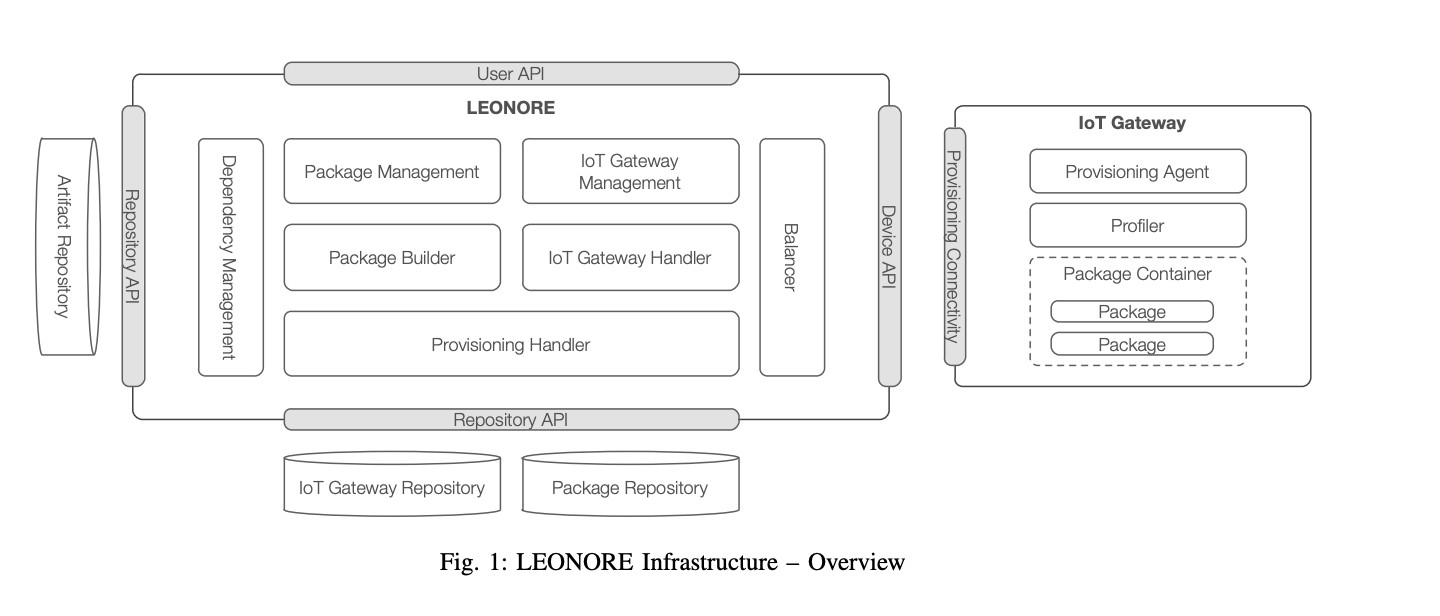
\includegraphics[width=0.8\textwidth]{resources/chapter-2/arsitektur-leonore.jpg}
  \caption{Arsitektur Leonore \parencite{vogler2015leonore}}
  \label{fig:arsitektur-leonore}
\end{figure}

Ilustrasi cara kerja LEONORE dapat dilihat pada gambar \ref{fig:sequence-leonore}. Berikut adalah cara kerja dari sistem LEONORE:
\begin{enumerate}
  \item Mengecek ketersediaan \textit{Artifact}.
  \item Mengambil \textit{Iot Gateway} sebagai grup yang akan di-\textit{deploy}.
  \item Mendelegasikan tugas \textit{deployment} ke setiap \textit{Gateway} IoT.
  \item Analisa kompatibilitas untuk setiap \textit{nodes}.
  \item Resolve \textit{dependency} dan membuat \textit{application package} sesuai dengan grup \textit{Gateway} IoT
  \item Menjalankan \textit{provisioning}
  \item Menunggu hingga setiap \textit{nodes} selesai lalu melakukan pengecekan untuk setiap \textit{nodes} hingga proses selesai
\end{enumerate}

\begin{figure}[ht]
  \centering
  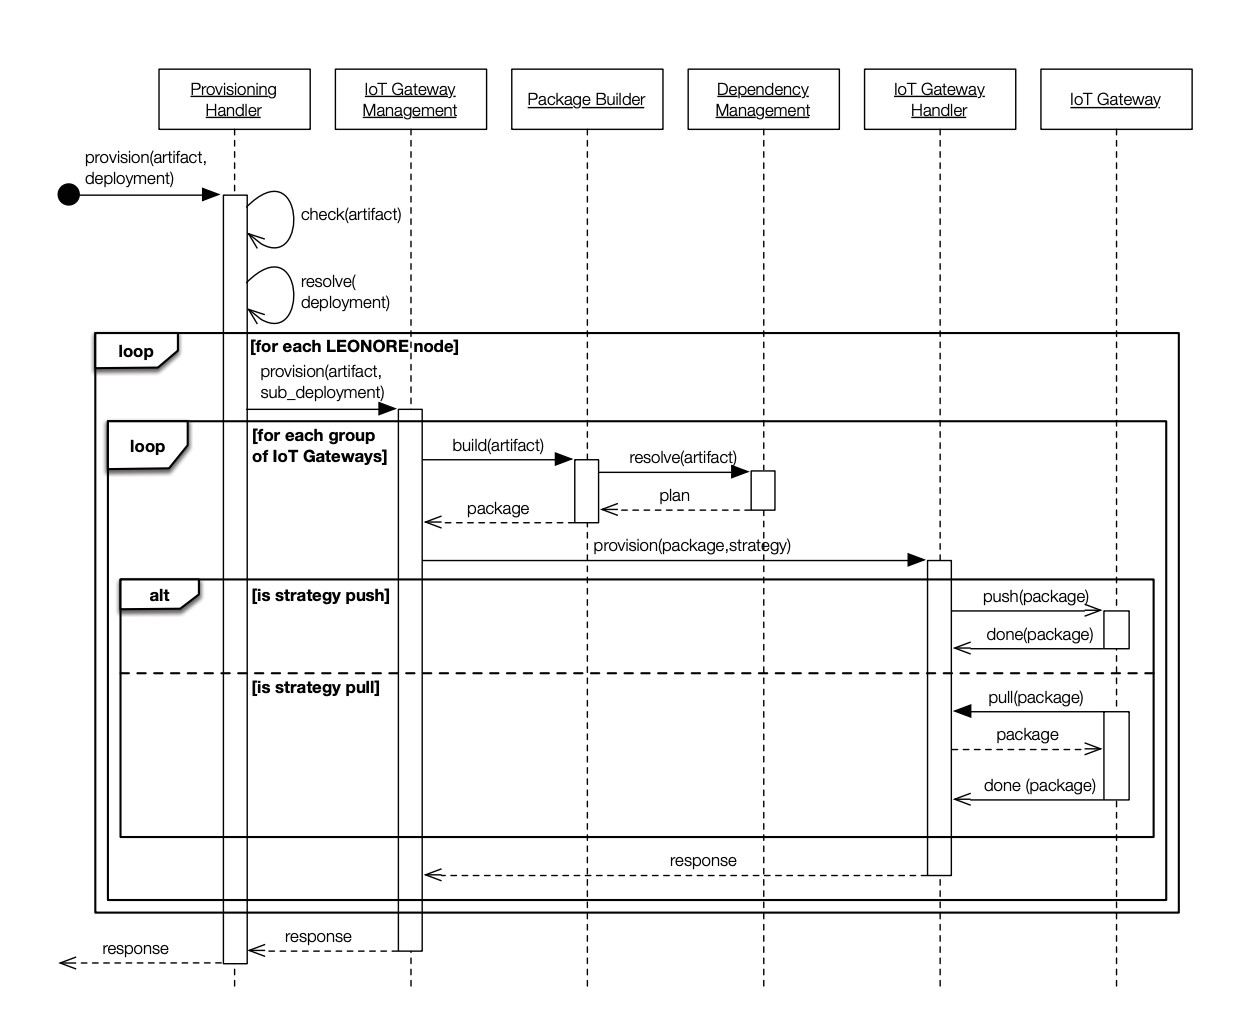
\includegraphics[width=0.8\textwidth]{resources/chapter-2/leonore-sequence.jpg}
  \caption{Sequence Diagram Proses \textit{Deployment} LEONORE \parencite{vogler2015leonore}}
  \label{fig:sequence-leonore}
\end{figure}

Untuk mengevaluasi kinerja LEONORE, dilakukan pengujian pada \textit{cloud} berisi 1000 perangkat yang divirtualisasi menggunakan \textit{docker}. Hasilnya, LEONORE dapat melakukan \textit{provisioning} seluruh perangkat dengan waktu yang \textit{reasonable}. Metode \textit{pull provisioning} menghasilkan latensi yang tinggi apabila dibandingkan dengan metode \textit{push} yang memberikan hasil cukup baik.